%%%%%%%%%%%%%%%%%%%%%%%%%%%%%%%%%%%%%%%%%%%%%%%%%%%%%%%%%%%%%%%%%%%%%%%%%%%%%%%%
%2345678901234567890123456789012345678901234567890123456789012345678901234567890
%        1         2         3         4         5         6         7         8

%\documentclass[letterpaper, 10 pt, conference]{ieeeconf}  % Comment this line out
                                                          % if you need a4paper
\documentclass[a4paper, 10pt, conference]{ieeeconf}      % Use this line for a4
                                                          % paper

\IEEEoverridecommandlockouts                              % This command is only
                                                          % needed if you want to
                                                          % use the \thanks command
\usepackage{epsf,graphicx}
\usepackage{latexsym,amssymb}
\usepackage{setspace,cite}

\overrideIEEEmargins
% See the \addtolength command later in the file to balance the column lengths
% on the last page of the document

% The following packages can be found on http:\\www.ctan.org
%\usepackage{graphics} % for pdf, bitmapped graphics files
%\usepackage{epsfig} % for postscript graphics files
%\usepackage{mathptmx} % assumes new font selection scheme installed
%\usepackage{times} % assumes new font selection scheme installed
%\usepackage{amsmath} % assumes amsmath package installed
%\usepackage{amssymb}  % assumes amsmath package installed

\title{\LARGE \bf
Superpixel flow
}

%\author{ \parbox{3 in}{\centering Huibert Kwakernaak*
%         \thanks{*Use the $\backslash$thanks command to put information here}\\
%         Faculty of Electrical Engineering, Mathematics and Computer Science\\
%         University of Twente\\
%         7500 AE Enschede, The Netherlands\\
%         {\tt\small h.kwakernaak@autsubmit.com}}
%         \hspace*{ 0.5 in}
%         \parbox{3 in}{ \centering Pradeep Misra**
%         \thanks{**The footnote marks may be inserted manually}\\
%        Department of Electrical Engineering \\
%         Wright State University\\
%         Dayton, OH 45435, USA\\
%         {\tt\small pmisra@cs.wright.edu}}
%}

\author{Juan Perez Rua% <-this % stops a space
\thanks{This work was supported by Technicolor SA}% <-this % stops a space
\thanks{Juan Perez Rua  is with Technicolor R\&D and the University of Burgundy,
        {\tt\small juanmanuel.perezrua@technicolor.com}}%
}


\begin{document}



\maketitle
\thispagestyle{empty}
\pagestyle{empty}


%%%%%%%%%%%%%%%%%%%%%%%%%%%%%%%%%%%%%%%%%%%%%%%%%%%%%%%%%%%%%%%%%%%%%%%%%%%%%%%%
\begin{abstract}

Superpixels and over segmentation techniques
became a widely used pre-processing stage for a
large number of machine vision applications, after the
original concept was introduced \cite{c1}. Superpixels are
traditionally used as performance booster for several
other techniques. However, it is still mostly related to
single frame processing \cite{c1}\cite{c10}\cite{c11}. In the search for
consistency in superpixel labeling through video,
some authors have proposed different techniques,
which go from simple extension to super-voxels\cite{c9}\cite{c11},
to more complicated approaches \cite{c8}. These
approaches, nonetheless, usually require a global
processing and knowledge of all (or several of) the
video frames beforehand. In this paper we propose a superpixel
matching technique which assumes a flow-like
behavior in the image sequences (natural video), and
propose an application for improving object segmentation in videos.


\end{abstract}


%%%%%%%%%%%%%%%%%%%%%%%%%%%%%%%%%%%%%%%%%%%%%%%%%%%%%%%%%%%%%%%%%%%%%%%%%%%%%%%%
\section{INTRODUCTION}

For some kind of video sequences and computer vision
applications the video consistency is not well preserved (I.e
long term tracking, moving camera videos, etc.). Usually,
the super-pixel labelling loses coherency between frames, 
even when computed as super-voxels. 
This means super pixel matching techniques offer some interest and can still be
explored. Some work have been done towards a
super-pixel based image comparison using the Earth
Mover’s Distance, by taking super pixels as bins of a
global histogram \cite{c2}. The label propagation or superpixel flow can be
achieved with this technique by selecting the super-
pixel in the second frame that maximize the flow
from each super-pixel in the first frame.
However, we look at the problem of super-pixel
propagation between a pair of frames, in terms of the
indexes of the already computed superpixelization in
both of them. Thus, the propagation means finding
the super-pixel label in the second frame that
correspond to a given label in the first frame. This
matching, however, has to comply with a set of
constraints. Firstly, two correspondent super-pixels
should be similar in terms of some appearance
feature, which most likely depends on the way the
superpixelization was performed (color, texture,
shape). Also, the super-pixel propagation should
maintain certain global homogeneity (at least for
super-pixels that belong to the same object). This is
because the super-pixel propagation or matching is
not completely a one-to-one combinatorial problem,
but more a “superpixel flow”. In this sense, it seems
natural that the problem of super-pixel propagation
could be solved with a discrete energy minimization
procedure. If the size homogeneity of the superpixels is maintained, 
it actually seems to share some of the properties of the
optical flow problem, with the difference that the
smoothness is usually a very strong constraint for the
last one. The strength of this smoothness prior relies
not only in the nature of the problem, but also
because it gives better cues towards an easy-to-
minimize global approach.


%%%%%%%%%%%%%%%%%%%%%%%%%%%%%%%%%%%%%%%%%%%%%%%%%%%%%%%%%%%%%%%%%%%%%%%%%%%%%%%%
\section{PROBLEM DEFINITION}

The objective of the super-pixel propagation is
therefore to find the best labeling $L$ for every superpixel $p$
(with $L_p \in {0,1,...N-1}$) between a pair
of frames ($I_{1}$,$I_{2}$), but holding a flow-like behavior.
   \begin{figure}[thpb]
      \centering
      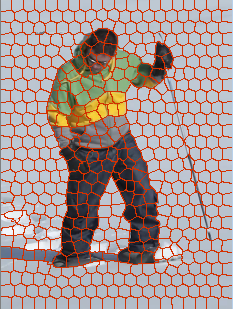
\includegraphics[height=0.22\textheight]{images/segmentation.png}
      \caption{SLIC super segmentation in the Snow Shoes sequence.}
      \label{figurelabel_segmentation}
   \end{figure}
Thus, the superpixelization should maintain certain
regularity in size within a single frame. Some super
pixel techniques can cope with this requirement \cite{c9}\cite{c10}.
For the experiments presented in this work, we prefer
the SLIC (Fig. \ref{figurelabel_segmentation}) method \cite{c9}, which usually gives
good results in homogeneity of the superpixelization.
The proposed steps to solve the propagation problem
assume this requirement is hold. For other kind of the
techniques, other approaches should be followed.

%\addtolength{\textheight}{-3cm}   % This command serves to balance the column lengths
                                  % on the last page of the document manually. It shortens
                                  % the textheight of the last page by a suitable amount.
                                  % This command does not take effect until the next page
                                  % so it should come on the page before the last. Make
                                  % sure that you do not shorten the textheight too much.

%%%%%%%%%%%%%%%%%%%%%%%%%%%%%%%%%%%%%%%%%%%%%%%%%%%%%%%%%%%%%%%%%%%%%%%%%%%%%%%%
\subsection{Energy Formulation}

Inspired by a large number of optical flow and stereo
techniques \cite{c7}\cite{c12}\cite{c13}, the super-pixel propagation can be
modeled with pairwise Markov Random Fields. If
the matching is performed with MAP inference, its
posterior probability is: 
\begin{equation}
 P(L|I_0,I_1) = \displaystyle \prod_{p \in \Omega} \mathrm{e}^{-D_p(L_p;I_0,I_1)} 
\prod_{p,q \in \mathcal{N}_p} \mathrm{e}^{-S_{p,q}(L_p;L_q)} 
\label{eq_prob}
\end{equation}

With $L$ the set of labels of the super pixels in $I_0$,
that match with those in $I_1$.
$ \mathcal{N}_p $ is a neighborhood of the
superpixel $p$, which defines its adjacency. Given this posterior probability,
the equivalent energy function can be directly obtained
by extracting the negative logarithm of the posterior,

\begin{equation}
E(L) = \displaystyle \sum_{p \in \Omega} -D_p(L_p;I_0,I_1) +
\sum_{p,q \in \mathcal{N}_p} -S_{p,q}(L_p,L_q)
\label{eq_energy}
\end{equation}

The terms $D$, and $S$ in \ref{eq_energy} stand for data and spatial as they
are popularly known in the MRF literature. The first
one determines how accurate is the labeling in terms
of consistency of the measured data (Color, Shape,
etc.). In the optical flow counterpart of this equation,
usually the data term correspond to the pixel
brightness \cite{c7}\cite{c5}. However, as superpixels are a set
of similar (or somehow homogenous) pixels, an
adequate color based feature can be a low binned
histogram or its average color. So it can be written 
more precisely as

\begin{equation}
D_p(L_p;I_0,I_1) = \rho(h(p),h(p'))
\label{eq_Dp}
\end{equation}

Where $h(p)$ and $h(p')$ are the histograms of the super-
pixel $p$ and its correspondent superpixel in the
second frame ($I_1$). $rho$ can be replaced by the Bhattacharyya
 distance. Note that the low binned histogram or
average color gives certain robustness against noise,
and slowly changing colors between frames.
The spatial term is a penalty function for horizontal
and vertical changes of the vectors that have origin in
the centroid of the super-pixel of the first frame and
end in the centroid of the super-pixel of the second
frame.

\begin{equation}
S_{p,q}(L_p,L_q) = \lambda(p)
  \sqrt{\frac{|u_{p_c}-u_{q_c}|}{\|p_c-q_c\|}+ \frac{|v_{p_c}-v_{q_c}|}{\|p_c-q_c\|}}
\label{eq_Spq}
\end{equation}
\begin{center}
 where, $ \lambda(p) = (\rho(h(p),h(p')))^2 $ \\
\end{center}

In \ref{eq_Spq} the operator $\rho$ has the same meaning as in the
data term \ref{eq_Dp}. The histograms distance is nonetheless
computed between super pixels $p$ and $q$, which belong to
the same neighborhood. The super pixels
centroids are noted as $q_c$ and $p_c$, and $u$ and $v$ are the
horizontal and vertical changes between centroids.
This term is usual in the MRF formulation and has a
smoothing effect in superpixels that belong to the
same object. It has to be observed that when two
superpixels are different, thus, more probable to be
in different semantic groups within the image, the
term $\lambda$ allows them to have
matches that do not hold the smoothness prior with the same strength. 
It has to be noted that the proposed energy function is
highly non-convex and robust.

\subsection{Energy Minimization}

A fair amount of work had been dedicated to
discrete optimization techniques in computer vision,
leading to a couple of well-defined and widely tested
approaches to solve the pairwise MRF of labels \cite{c3}\cite{c4}.
However, some of the approaches restrict the
construction of the spatial term, and/or enforce
limitations in the number of labels \cite{c3}.
Because of the high amount of possible labels for 
each element in the proposed approach, the use of the
Fusion Moves \cite{c7} technique seems to be well suited.
This algorithm employs the Quadratic Pseudo-
Boolean Optimization (QPBO) graph-cut, to combine
incremental sets of proposal labeling, resulting a semi-
globally-optimal solution \cite{c4}.
Thus, the minimization starts by proposing a set of
possible solutions, and iteratively merge them with
the QPBO graph-cut technique. \\
The possible solutions that can be given depend on the kind of
problem that is intended to be solved. For example, in
stereo super-pixel matching, some assumptions
related to the cameras organization can be made to
generate solutions.
In a more generic sense, other assumptions can be
made towards option generation. For instance, for a
given super-pixel in the initial frame, in the second
frame the corresponding matching would be the most
similar one in terms of color, or the most similar un
terms of shape, or the spatially closer super-pixel.
More proposal solutions can be added by defining a
neighborhood in the second frame and select random
pairs from every neighborhood of every super-pixel
in the first frame. This is more suitable for problems
where the images are extracted from the same video
sequence. It is interesting to notice that different
assumptions for this neighborhood can lead to a
technique for generic image based retrieval, where
the total cost of matching can be used as metric.

\section{EXPERIMENTAL RESULTS}
The Fig. \ref{figurelabel_matches} shows some examples of superpixel
matching with the presented method. It can be seen
that the matching performs well even in difficult
cases, like the hands in the top row. It has to be noted
as well that even in super-pixels where there is a lack
of texture, there is correct matching. This seems to be
the effect of enforcing the regularization between
super-pixels that are close, but are also similar to
each other.

   \begin{figure}[thpb]
      \centering
      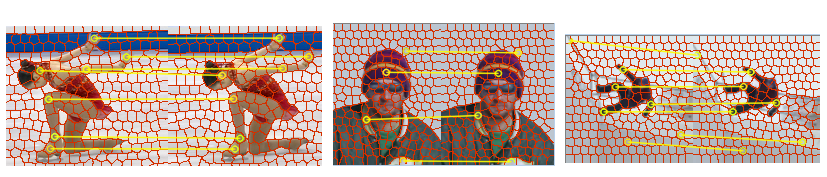
\includegraphics[height=0.33\textheight]{images/matches.png}
      \caption{The yellow lines show selected super-pixel
		matching between pairs of subsequent frames in a video
		with the proposed method. The video frames go from right
		to left.}
      \label{figurelabel_matches}
   \end{figure}
   
   
\subsection{Superpixel propagation for object segmentation in videos}
The GrabCut algorithm proposed in \cite{c14}, offers a good deal in terms of
background-foreground separation from user interaction. A technique like this, however,
performs very well in still images, but it may not be well adapted for sequential videos, 
The GrabCut works by implementing an iterative graph cut based 
minimization to separate regions according to appearance information, that can be
extracted from the user interaction. This interaction, however, could be minimized in videos,
given the extra information that offers the flow of the sequence.
Some authors had approached the GrabCut or similar
graph based segmentation techniques in sequential
videos, to propagate a consistent segmentation \cite{c15}.
However, some more work on reducing user interaction given the extra flow-like information
that video sequences offer is still needed.
We propose to combine the presented super pixel
propagation as an automatic method to initialize the
Grabcut (or similar) algorithm to perform object
segmentation through frames in a video sequence. \\

The idea is to track (or more exactly, match) super
pixels that are labeled as foreground, thanks to an
object tracker initialization. Thus, the super pixels
that are initially outside the ROI, can be propagated through the sequence,
and if they fall into the ROI of the next frame, they
can be safely labeled as foreground again. The process is
repeated for any labeled super-pixel through the
video. Having several labeled super pixels can reduce
widely the necessity for user interaction in
subsequent frames. Thus, to perform object
segmentation in a full video sequence, the required
user interaction would only be the initial bounding
box. Moreover, a fully automatic approach can be
obtained if a reliable object detector is available.

Fig. \ref{figurelabel_walking} shows how the initialization of a
tracker and a superpixelization provides information
for better background-foreground separation. The
background-foreground models are updated as the
frames go on, giving more robustness for sequential
propagation of the segmentation. The method is tested in the 
Walking Couple sequence,
by allowing only a small amount of iterations in the
graph based segmentation. Observe how the contour
in the man’s head is correctly delineated when
another person’s head occludes part of it. In this case,
the super-pixels that belong to the woman’s face
were correctly propagated and thus, labeled as
background. \\
   \begin{figure}[thpb]
      \centering
      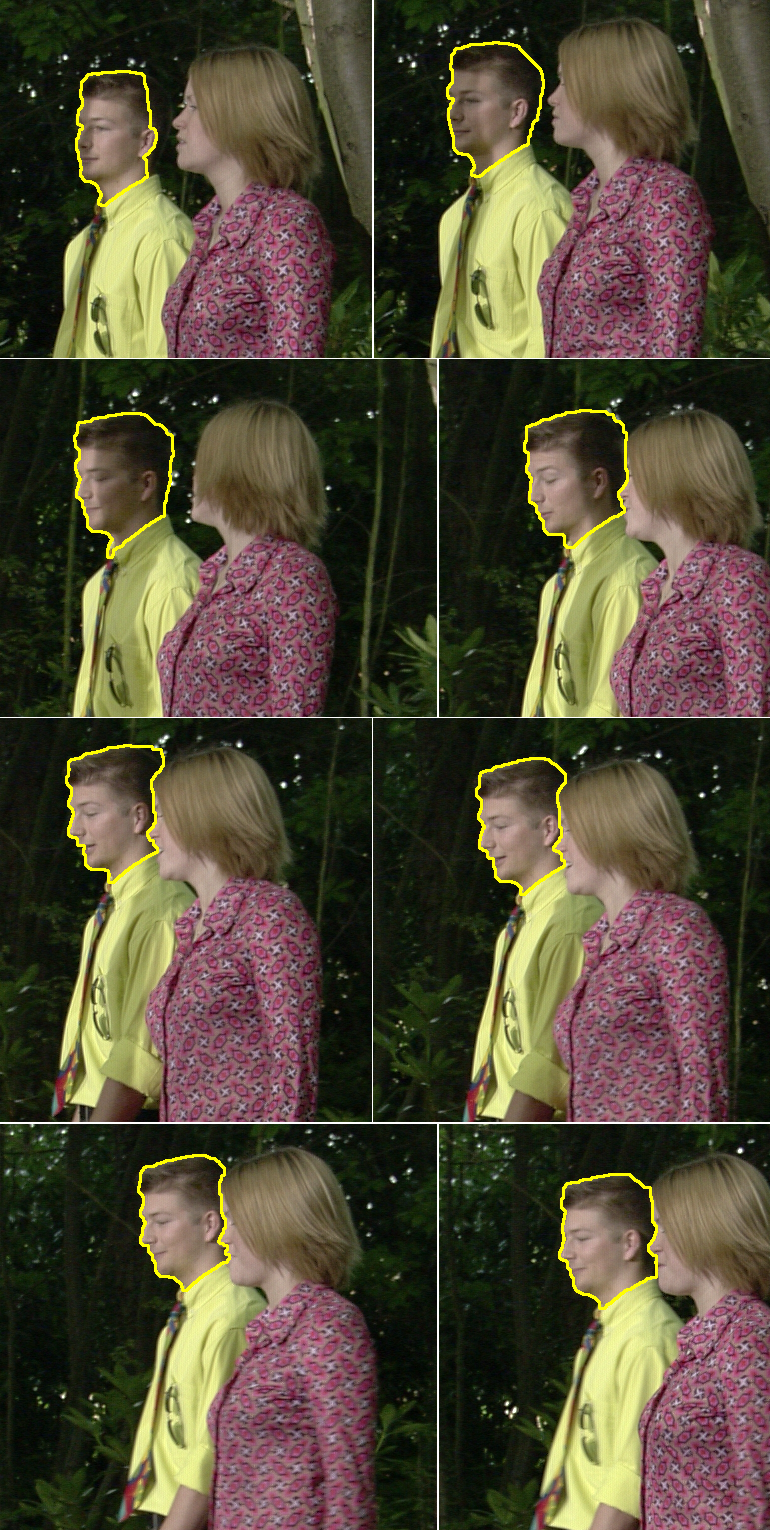
\includegraphics[height=0.66\textheight]{images/Sequence2.png}
      \caption{Segmentation through the sequence “Walking
	       Couple” (Yellow contour) initialized in the man’s head.}
      \label{figurelabel_walking}
   \end{figure}

In order to understand the effect of including super-
pixel propagation in a video sequence for object
segmentation, some results are shown in the Fig.
\ref{figurelabel_comp}. For these experiments only one iteration is
allowed in both grab-cuts initialized with only the
tracker, and the one performed with the super-pixel
propagation. Observe that in general, the contour
delineated is usually better in terms of precision and
stability for the later one.

   \begin{figure}[thpb]
      \centering
      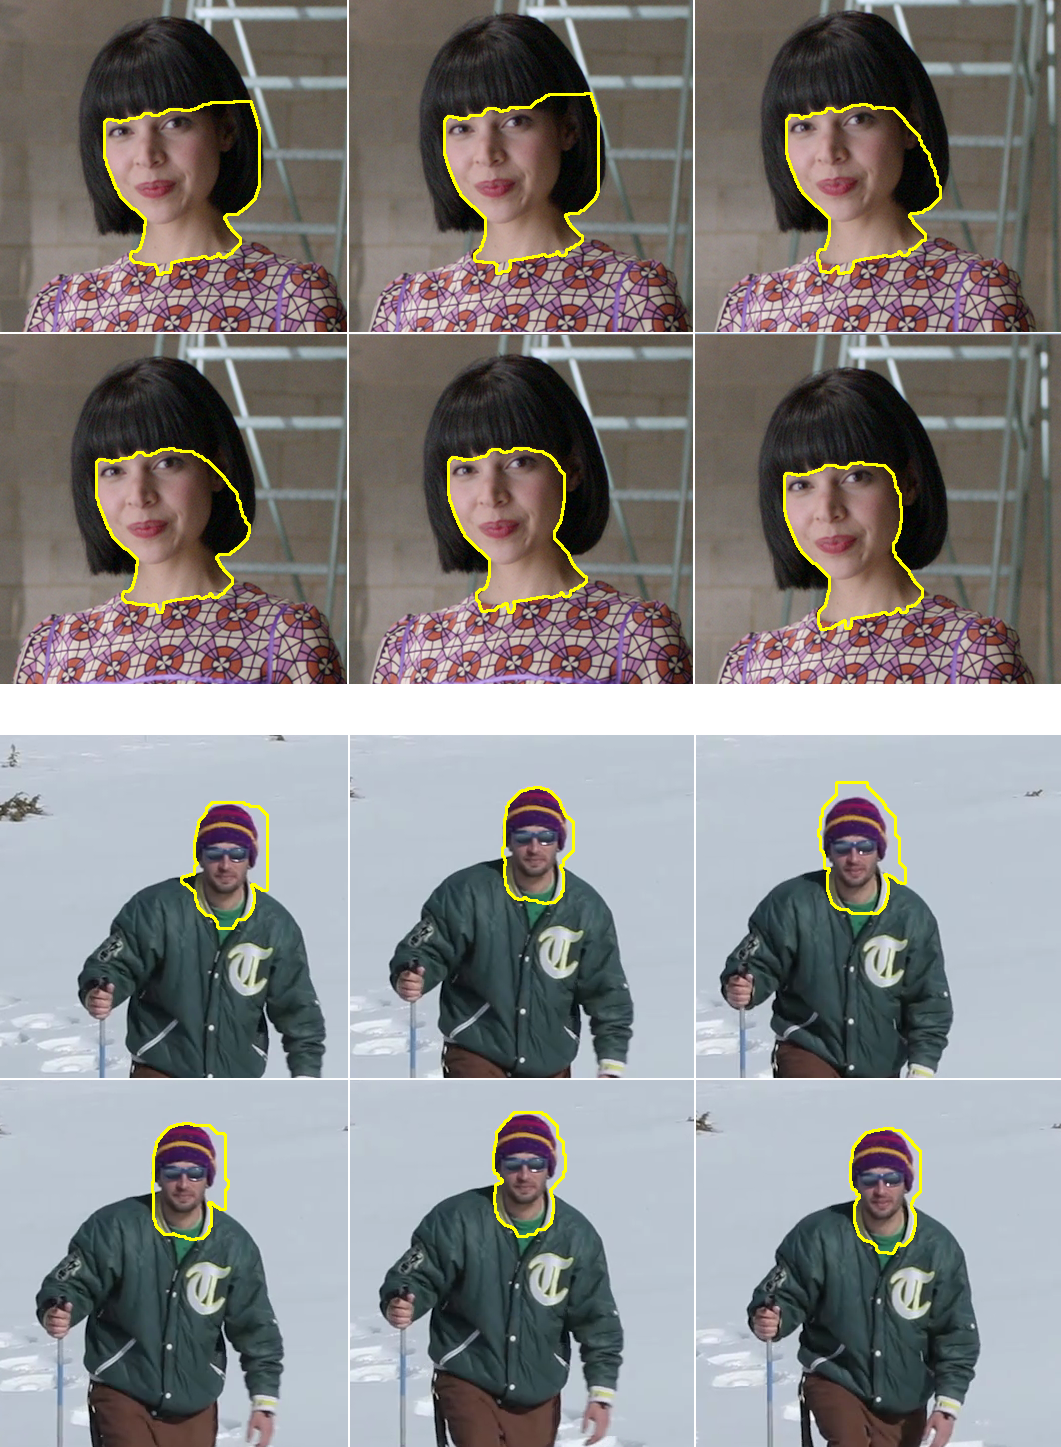
\includegraphics[height=0.4\textheight]{images/Compare.png}
      \caption{Face segmentation in the “Amelie Retro” and the
	      “Snow shoes” sequences in three different frames. For each
	       group, the Top Row: One-iteration window-based grabcut;
	       and the Bottom Row: One-iteration grabcut with super pixel
	       propagation.}
      \label{figurelabel_comp}
   \end{figure}
   
%%%%%%%%%%%%%%%%%%%%%%%%%%%%%%%%%%%%%%%%%%%%%%%%%%%%%%%%%%%%%%%%%%%%%%%%%%%%%%%%
\section{CONCLUSIONS}

A method for super-pixel matching in a flow-like
behavior had been presented. We may call it superpixel propagation, or super-pixel flow. This
technique shows robustness in the labeling of the
matches, and seems to be able to improve the results
for object segmentation in video sequences when
using the Grab-cut algorithm. Another motivation for
this technique, however may be as initialization of
optical flow techniques, to obtain more robust results
due to a good initial guess for energy minimization
methods. This has to be looked at more deeply in future work.


%%%%%%%%%%%%%%%%%%%%%%%%%%%%%%%%%%%%%%%%%%%%%%%%%%%%%%%%%%%%%%%%%%%%%%%%%%%%%%%%

\begin{thebibliography}{99}

\bibitem{c1}
J. Malik and X. Ren, Learning a classification model for segmentation, {\it Computer Vision, International Conference}, 2003.

\bibitem{c2}
S. Boltz; F. Nielsen and S. Soatto, Earth mover distance on superpixels{\it International Conference on Image Processing}, 2010.

\bibitem{c3}
E. Boros; P. Hammer and G. Tavares, Preprocessing of unconstrained quadratic binary optimization {\it RUTCOR}, 2010

\bibitem{c4}
E. Boros and P. Hammer, Pseudo-boolean optimization{\it Discrete applied Mathematics.}, 2002

\bibitem{c5}
B. Horn and B. Schunck, Determining Optical Flow{\it Artificial Intelligence}, 1981

\bibitem{c6}
H. Ishikawa and P. Bouthemy, Multimodal estimation of discontinous optical flow using Markov random fields{\it TPAMI.}, 1993

\bibitem{c7}
V. Lempitsky, S. Roth and C. Rother, Fusion Flow: Discrete-Continuos optimization for optical flow estimation{\it Computer Vision and Pattern Recognition}, 2008

\bibitem{c8}
M. Reso and J. Jachalsky, Temporally Consistent Superpixels{\it International Conference Computer Vision.}, 2011

\bibitem{c9}
R. Achanta; A. Shaji; K. Smith; Aurelien Lucchi; P. Fua and S. Susstrunk SLIC Superpixels compared to state of the art superpixel methods{\it Discrete applied Mathematics.}, 2002

\bibitem{c10}
F. Perbet and A. Maki, Homogeneus superpixels from random walks{\it MVA.}, 2011

\bibitem{c11}
C. Xu and J.J. Corso. Evaluation of super-voxel methods for early video proccesing. {\it Computer Vision and Pattern Recognition}. 2012.

\bibitem{c12}
A. Shekhovtsov, I. Kovtun and V. Hlavac. Efficient MRF deformation model for non-rigid image matching. {\it Computer Vision and Pattern Recognition}. 2007.

\bibitem{c13}
J. Sun, N.N Shen and H.Y. Shum. Stereo matching using propagation belief. {\it TPAMI}. 2003.

\bibitem{c14}
C. Rother, V. Kolmogorov and A. Blake. Grabcut: Interactive foreground extraction using iterated graph cuts. {\it SIGGRAPH}. 2004.

\bibitem{c15}
L. Yang, Y. Guo, X. Wu and X. Wang. A new video segmentation approach: Grabcut in local window. {\it Soft Computing and Pattern Recognition}. 2011.

\end{thebibliography}

\end{document}
